\appendix
\section{Code}

\begin{listing}[h]
    \centering
    \begin{minipage}{0.9\textwidth}
        \begin{minted}[frame=single, fontsize=\footnotesize]{python}
def remove_noise(text: str) -> str:
    # Remove URLs
    text = re.sub(r'http\S+|www\.\S+', '', text)
    # Remove emails
    text = re.sub(r'\b[A-Za-z0-9._%+-]+@[A-Za-z0-9.-]+\.[A-Za-z]{2,}\b', '', text)
    # Remove digits
    text = re.sub(r'\d+', '', text)
    # Remove punctuation and special characters (excluding spaces)
    text = re.sub(r'[^\w\s]', '', text)
    # Remove extra spaces
    text = re.sub(r'\s+', ' ', text).strip()

    return text
        \end{minted}
    \end{minipage}
    \caption{Preprocessing function}
    \label{lst:preprocessing}
\end{listing}

\section{Visualizations}

\begin{figure}[h]
    \centering
    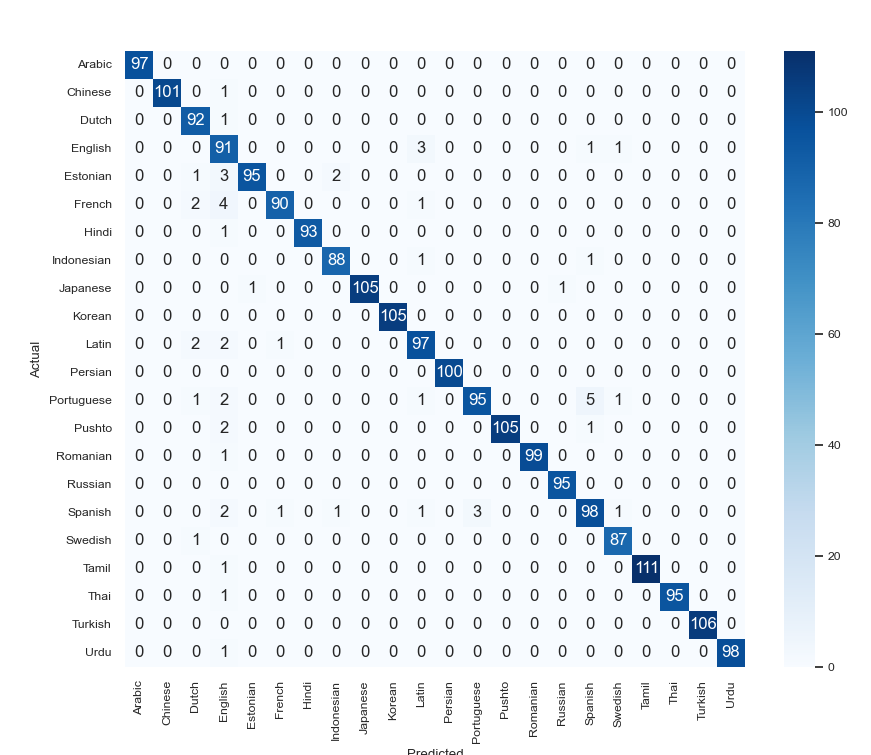
\includegraphics[width=0.8\textwidth]{figures/svm_char_unigram_val_set_matrix.png}
    \caption{Confusion matrix of the SVM model trained on the character unigram features}
    \label{fig:matrix_svm_char_unigram}
\end{figure}

\begin{figure}
    \centering
    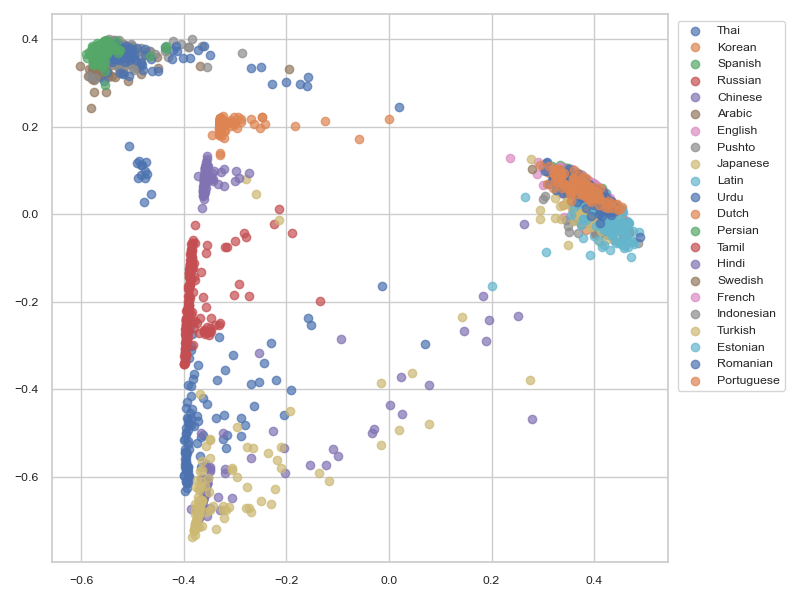
\includegraphics[width=0.9\textwidth]{figures/svm_char_unigram_val_set_pca.png}
    \caption{PCA visualization of the SVM model trained on the character unigram features}
    \label{fig:pca_svm_char_unigram}
\end{figure}

\begin{figure}
    \centering
    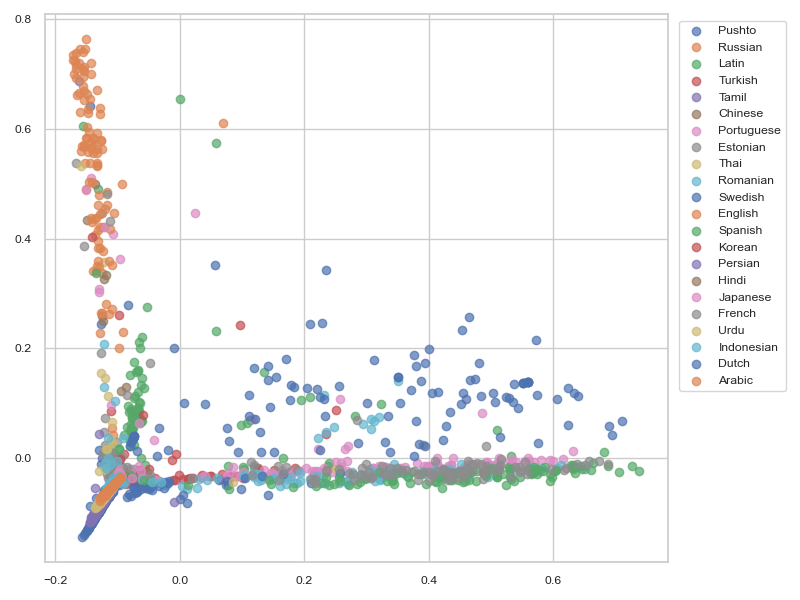
\includegraphics[width=0.9\textwidth]{figures/svm_word_unigram_val_set_pca.png}
    \caption{PCA visualization of the SVM model trained on the word unigram features}
    \label{fig:pca_svm_word_unigram}
\end{figure}


